\section{Comunicación vehicular}\label{section:comunicacion_vehicular}
Los \gls{rsu} y \gls{obu} son los encargados de proveer la información sobre posiciones
de los vehículos a motor a la \emph{Nube de Conductores}. Cada uno se ha implementado
mediante un router Linkbird-MX y un ordenador portátil conectado a través de un conector
RJ-45; aunque en un escenario real se puede prescindir del ordenador portátil. Cada
uno tiene una aplicación Java ejecutándose, cada uno con una misión diferente. Para
poder hacer uso de las funciones que provee el router Linkbird-MX, se emplea la \gls{api}
provista por NEC. Así mismo, se utiliza Ant para facilitar el despliegue de las
aplicaciones.

\subsection{Unidad de a bordo}
Cada vehículo posee un \gls{obu} integrado: formado por un router, una unidad \gls{hmi}
y, si se desea, puede poseer una unidad \Gls{obd-ii} [\ref{apendice:open-xc}]. Un GPS
está conectado al router para recibir la posición, velocidad y dirección del vehículo.
A través del canal Broadcast de la red \emph{IEEE 802.11p} se envía la información
recibida sobre el vehículo al que está conectado a la \gls{rsu}, en forma de pequeños
beacons. El funcionamiento de la aplicación consiste en:
\begin{itemize}
	\item Obtener la posición del vehículo realizando peticiones al router.

	\item Mandar periódicamente las posiciones a través de broadcast.

	\item Escuchar los mensajes que mandan las RSU.

	\item Ofrecer y proveer al usuario la información de los mensajes a través del HMI.
\end{itemize}

Para proveer información al conductor se emplea el \gls{hmi}, el cual consiste en un
ordenador de a bordo con sistema operativo Android; adicionalmente, se puede conectar
al \Gls{obd-ii} por el puerto serie que provea el dispositivo, para obtener información
del vehículo; como por ejemplo, el estado de los neumáticos. El \gls{hmi} puede tener
instaladas varias aplicaciones, para poder proveer información sobre los ciclistas en
carretera se ha desarrollado una app.

Esta aplicación se encarga de procesar los mensajes recibidos por el \gls{obu}. Para
ello, se emplea una conexión Bluetooth para conectar ambos dispositivos. Una vez
recibe un mensaje, la aplicación muestra mediante un icono la posición del ciclista,
y produce una alerta cuando existe peligro de colisionar con el ciclista [Figura
\ref{figure:HMI}]. Las posiciones de los ciclistas son almacenadas en el vehículo
durante un período de 30 segundos; según llegan las nuevas posiciones desde la nube,
se van actualizando. Pasado ese tiempo, los registros que no hayan sido refrescados son
eliminados; esto significa que los nodos han dejado de transmitir.

Para crear el servidor Bluetooth que envíe los mensajes recibidos por el \gls{obu} a la
aplicación instalada en el \gls{hmi}, se ha utilizado la librería libre Bluecove. Se ha
creado un servicio con UUID personalizado en el cual se envían los mensajes que se han
recibido en el \gls{obu} y deben ser mostrados al usuario.

\begin{figure}[H]
	\begin{center}
		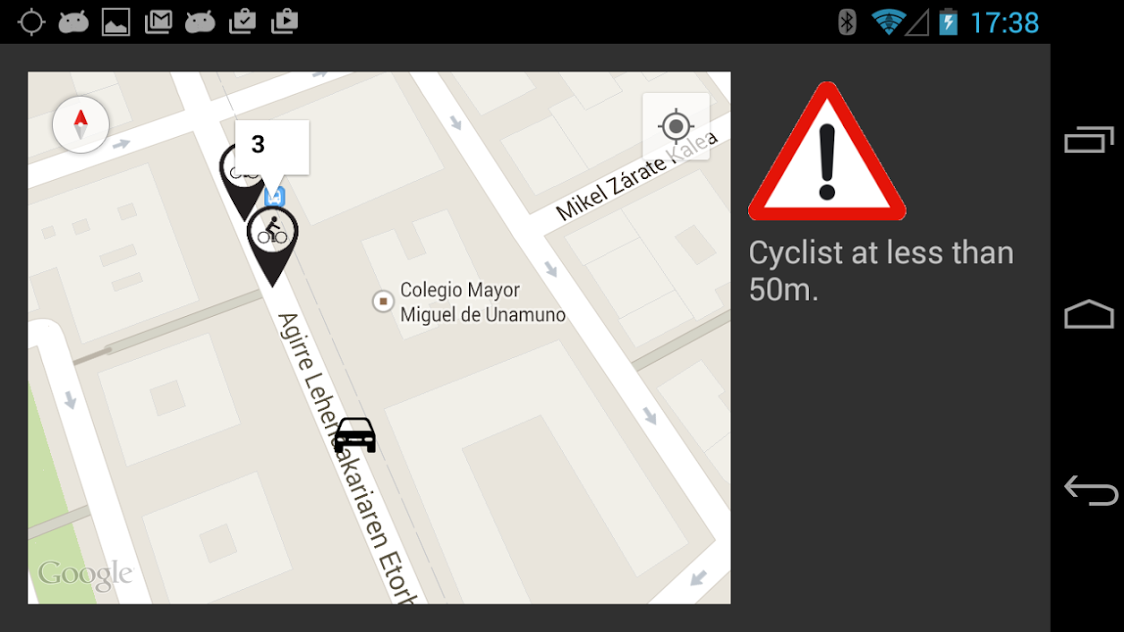
\includegraphics[scale=0.4]{HMI}
		\caption{UI de la aplicación instalada en el HMI}
		\label{figure:HMI}
	\end{center}
\end{figure}

\subsection{Unidad de carretera}
Las \gls{rsu} se encuentran desplegadas en las diferentes infraestructuras de la
carretera. Cada \gls{rsu} está formada por: un router, ordenador portátil y Modem-USB
que provea conexión a una red móvil. Actúa como puente entre las \gls{obu} instaladas
en los vehículos y la nube. Cuando se despliegue el sistema, es necesario conectar
primero tanto el cable procedente del router como el Modem-USB, seguidamente hay que
establecer que los mensajes procedentes de la red vehicular empleen la interfaz eth0,
y los mensajes que viajan a Internet empleen la interfaz wlan0; esto se puede hacer
mediante la herramienta \"routes\" que proporciona cualquier sistema GNU/Linux. El \gls{rsu}
escucha y escribe a través de dos canales:
\begin{enumerate}
	\item En el canal \gls{lte} recibe los mensajes \Gls{http/1.1} que provienen de la
	Nube de Conductores, así como envía las posiciones de los vehículos a la nube. Un
	servicio web posibilita la gestión de estos mensajes; el formato es igual que el
	explicado en la sección \ref{ssection:FormatoMensajesNC}.

	\item Escucha el canal IEEE 802.11p los mensajes que son enviados por los vehículos,
	y los redirige a la nube a través de mensajes \Gls{http/1.1}.
\end{enumerate}

Al recibir un mensaje el \gls{rsu} se comporta de la siguiente forma:
\begin{enumerate}
	\item Se comprueba que el formato del mensaje es correcto. Si no lo es, se descarta.

	\item Lectura del campo \"TYPE\" del mensaje. Dependiendo de su contenido se aplica
	un proceso diferente: el mensaje puede ser retransmitido a través de Broadcast, se
	puede mostrar una notificación en un panel informativo en carretera...
\end{enumerate}

Una propuesta para añadir funciones adicionales consiste en conectar el \gls{rsu} a
elementos informáticos que pueden existir en la carretera, por ejemplo los paneles
informativos, y al enviar un mensaje desde la Nube de Conductores a una \gls{rsu} en
concreto se pueda muestra la información deseada.
